% !TEX root = ../main.tex

%\chapter{\label{chapitres:perspectives} Perspectives}
\chapter{\label{section:conclusion}Conclusion}

% In this article, we have presented an experimental approach to characterize relevant aspects of the memory consumption to their sensitivity to memory interferences.
% We have introduced a set of microbenchmarks allowing us to reproduce a wide range of memory consumptions, both in nature and intensity, at a sufficiently large scale to use machine learning techniques.
% We have put in evidence the lack of precision of a purely quantitative characterization of memory consumption.
% In response, we have defined qualitative metrics quantifying the type of accesses, their interleaving, locality, or their impact on application progress.
% We have developed a tool to measure those aspects that also capture high resolution profiles allowing us to clearly identify distinct consumption behaviors in an application.
% Finally, we have used our microbenchmarks and our characterization to infer the overhead suffered by applications of the \textsc{MiBench} and the \textsc{PARSEC} suites.
% Results show a significant improvement of quality prediction compared to a purely quantitative characterization, showing the relevance of our metrics and the representativity of our microbenchmarks.

% In the future, we will explore several directions to improve this work.
% The first one is to build a set of conservative predictor that does not allow underestimations.
% This can involve the development of specific inference algorithms or new interference models incorporating our characterization.
% The second direction is to widen the scope of consumption behavior covered by our microbenchmarks and to find new relevant metrics.
% Finally, the last direction we want to explore is the automation of measure points placement, using computer vision techniques and code analysis.

% Résumé des contributions

Ce chapitre conclut ce document.
Nous y récapitulons les contributions apportées par nos travaux.
Nous tirons ensuite des conclusions de nos résultats.
Nous évoquons, enfin, les différentes perspectives qui s'offrent à nous pour améliorer l'approche que nous avons proposée.

% Ce chapitre conclue ce document. 
% En premier lieu, nous y faisons un résumé des contributions apportées par nos travaux.
% En deuxième lieu, nous exprimons les conclusions que nous pouvons tirer de nos travaux.
% Finalement, en troisième lieu, nous présenterons les perspectives d'amélioration s'offrant à nous.

\section{Résumé des contributions}

% Les interférences dues aux partage de matériel dans les processeurs multi-coeurs COTS est l'un des principaux obstacles à l'adoption de ces processeurs dans les systèmes embarqués temps-réels.
% L'ampleur des retards induits par ce phénomène s'avère difficile à quantifier, principalement à cause de l'opacité et de la complexité du matériel considéré.
% Dans ce document, nous nous sommes penché sur l'étude des aspects comportementaux des applications pouvant causer une sensibilité plus ou moins grande à ce problème.
% Nous y avons fait plusieurs contributions.
Au fil de ce document, nous avons produit une approche pour l'inférence du surcoût temporel induit par les interférences à partir d'une caractérisation du comportement en isolation.
La figure~\ref{fig:solution} illustre les différents éléments constituant cette approche, ainsi que les chapitres où ils sont définis (ou mis en œuvre).
% Les différents élements constitutifs de cette approche, ainsi que les chapitres où ils sont définis (ou mis en oeuvre) est illustré par la figure~\ref{fig:solution}.
%L'absence des chapitres 2 et 3 sur cette figure est normale, ceux-ci exposant le contexte technique dans lequel nous évoluons et non notre approche.
Les chapitres 2 et 3 n'apparaissent pas sur cette figure, car ils exposent respectivement le contexte technique et un état de l'art de la gestion d'interférences dans les systèmes temps-réels.

\begin{figure}
	\centering
	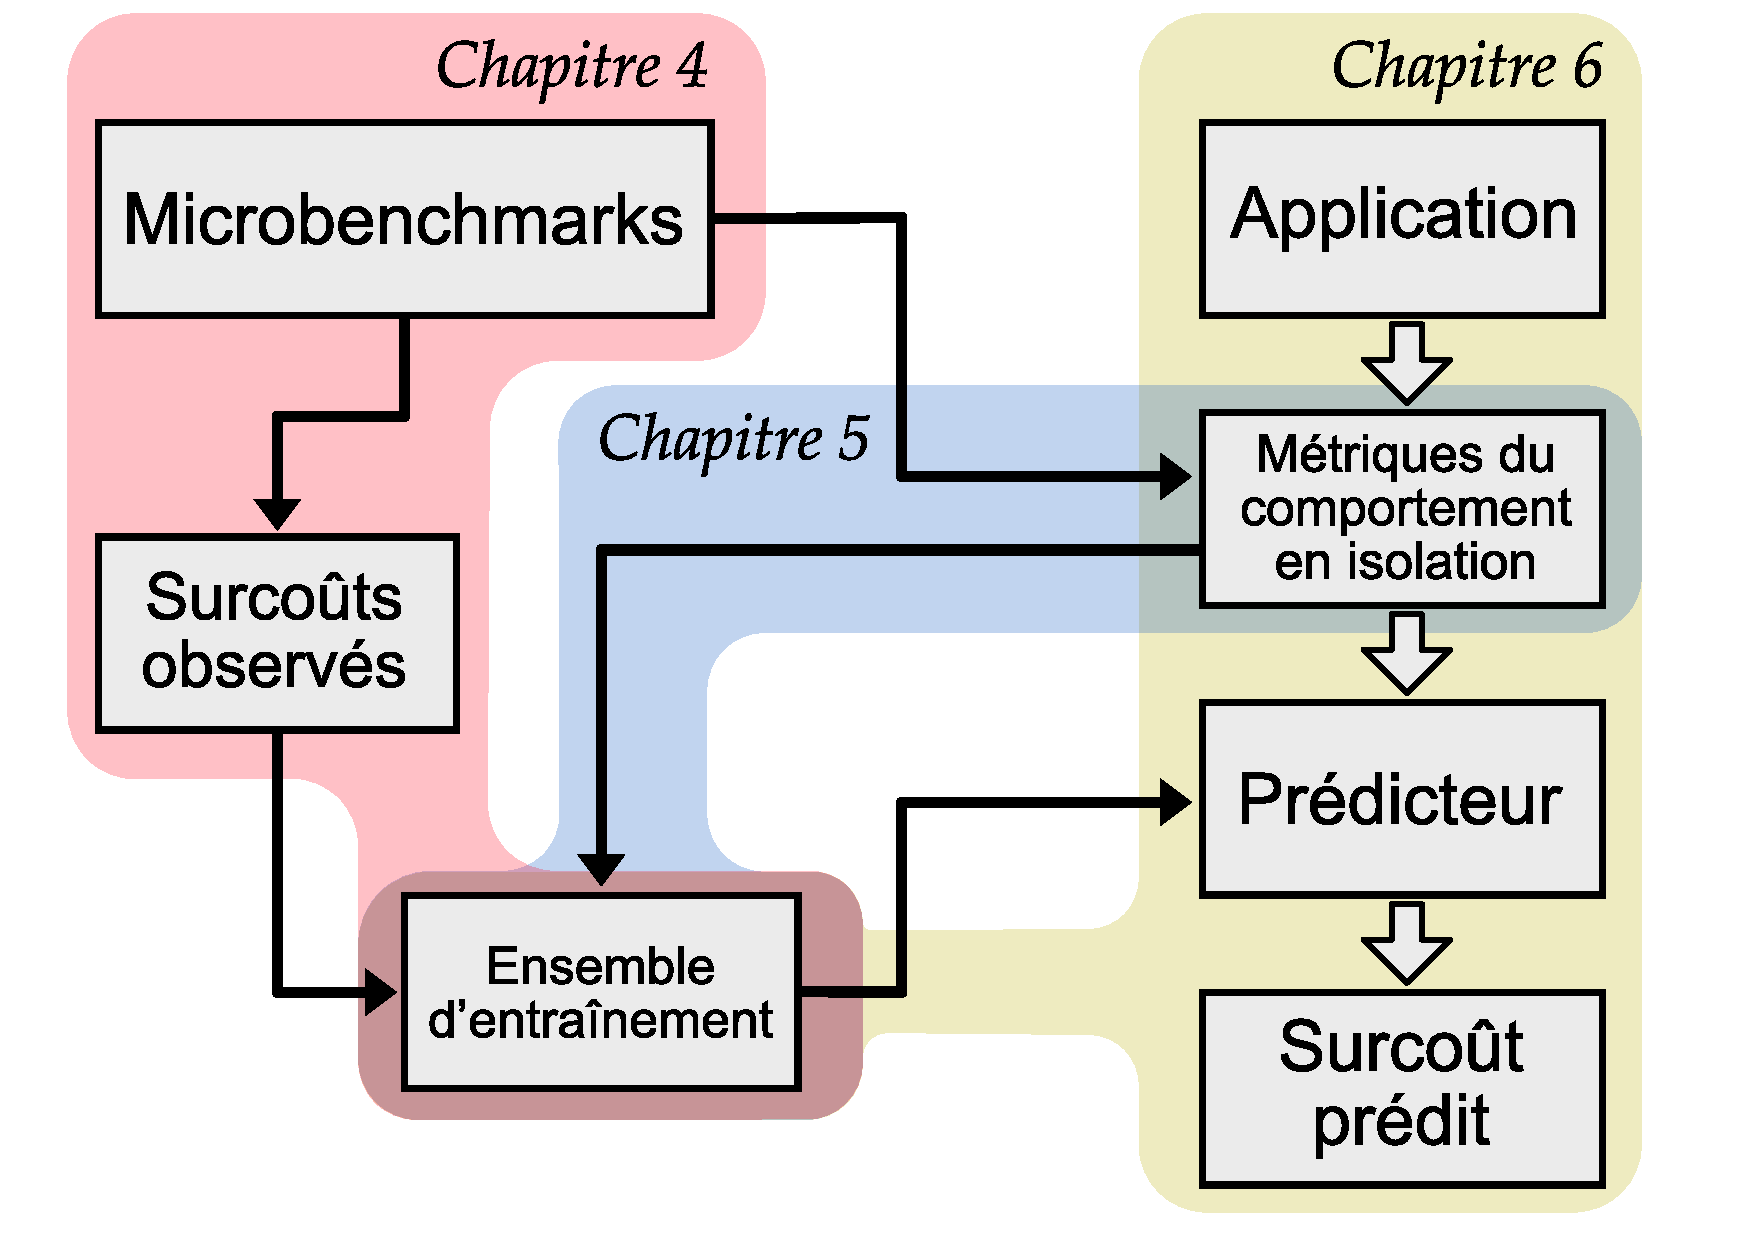
\includegraphics[width=0.75\linewidth]{solution-v2.pdf}
	\caption{\label{fig:solution}Architecture globale du mécanisme d'inférence défini dans nos travaux}
\end{figure}

Le chapitre 4 expose une étude de grande ampleur traitant de l'impact des interférences sur une cible multi-cœur COTS largement utilisée dans l'industrie.
%Dans le chapitre 4, nous avons présenté une étude de grande ampleur sur l'impact des interférences que l'on peut observer sur une cible multi-coeur COTS couramment utilisée dans l'industrie.
Pour conduire cette étude, nous avons développé un ensemble de microbenchmarks permettant de reproduire un grand nombre de comportements d'accès différents, variant aussi bien en \emph{nature} qu'en \emph{intensité}.
Cette suite étend des microbenchmarks existants tels que \textsc{STREAM}, en introduisant des paramètres permettant de contrôler leur comportement d'accès à la mémoire.
Ces paramètres sont déterminés à l'aide d'une  représentation événementielle des accès à la mémoire que nous avons préalablement introduite.
Si les résultats de cette première étude confirment que la sensibilité aux interférences est fortement corrélée à l'intensité du trafic, ils mettent aussi en évidence une forte influence de la nature des accès.
Notons que les microbenchmarks nous ont permis de constituer un ensemble de données nécessaire à la suite de nos travaux reposant sur des approches d'apprentissage automatique, comme le montre la figure~\ref{fig:solution}.

Dans le chapitre 5, nous nous sommes penchés sur la caractérisation des comportements applicatifs.
Le but étant alors de déterminer un ensemble de métriques, permettant de mesurer \emph{à priori} la sensibilité d'une application à la contention mémoire.
Parmi les métriques proposées, nous distinguons les métriques \emph{quantitatives} quantifiant l'intensité du trafic généré par les applications des métriques \emph{qualitatives} distinguant leur nature.
Dans cette deuxième étude, nous montrons qu'une caractérisation purement quantitative ne permet pas d'évaluer finement la sensibilité aux interférences, montrant ainsi la nécessité des métriques qualitatives.

Certaines métriques qualitatives que nous avons définies ne sont pas mesurables directement par des moyens classiques.
Nous avons résolu ce problème en nous appuyant sur une simulation de la représentation événementielle introduite dans le chapitre 4.
Pour ce faire, nous avons développé un prototype de profileur dans le framework d'instrumentation binaire dynamique \textsc{Valgrind}.
En plus de permettre la mesure de métriques qualitatives, ce profileur offre la possibilité de générer des profils en haute résolution de l'activité mémoire, permettant notamment d'identifier des phases caractéristiques.
Nous avons ainsi pu utiliser l'outil de profilage pour découper des applications issues des suites \textsc{MiBench} et \textsc{PARSEC}  en phases homogènes. % TODO phases identiqeus 

Enfin, dans le chapitre 6, nous utilisons les données issues de nos microbenchmarks pour prédire le retard subi par des applications à partir de métriques caractérisant leur comportement en isolation.
Cette prédiction repose sur des forêts aléatoires, un algorithme d'apprentissage automatique, entraîné avec des données associant des comportements en isolation à des surcoûts observés.
En plus de fournir une estimation du retard, ces prédicteurs nous permettent d'évaluer la pertinence des différentes métriques définies dans le chapitre 5.
En comparant la précision des prédictions obtenues en employant tel ou telle métrique, on observe un gain significatif de précision apporté par les métriques qualitatives.
L'erreur quadratique moyenne de l'ensemble de tests pouvant être réduite jusqu'à 61,2\%.
% Cela indique que ces métriques sont pertinentes pour la caractérisation des interférences.

% Pour cela, nous évaluons la précision d'algorithmes d'apprentissages automatiques pour prédire à priori le retards subi par des applications de tests en fonction de différentes caractérisation de leur comportement en isolation.
% Les prédicteur étant entrainés avec des données issus de nos microbenchmarks.
% Nous avons ainsi pu montrer que les métriques qualitatives que nous avons défini permettait d'améliorer significativement la qualité de prédiction.

% Étude du phénomène
% Microbenchmarks
% Caractérisation
% Inférences

\section{Conclusions de la thèse}
Comme nous avons pu le voir dans le chapitre 3, le problème des interférences est un obstacle majeur pour l'adoption des processeurs multi-cœurs COTS dans les applications critiques.
Ce problème est l'objet d'un grand nombre de publications scientifiques.
Les expériences conduites dans le cadre de nos travaux confirment que l'impact de ces interférences ne peut être négligé, dans la mesure où le prendre en compte conduirait à perdre tout le gain apporté par le multi-cœur.
% Ils montrent aussi qu'une approche générique, c'est à dire correspondant au pire retard observé quelque soit les applications
% En effet, il peut être tel, que les prendre en compte conduit à une utilisation moindre du matériel que si le système était mono-cœur.
Le défi est alors de pouvoir utiliser le matériel en étant suffisamment performant pour tirer parti du parallélisme.

Il est donc nécessaire de considérer individuellement chaque application en caractérisant leur comportement au travers de métriques spécifiques.
%Nous avons montré que l'on peut obtenir une assez bonne estimation du retards subi par des applications quelconques en nous basant uniquement sur des microbenchmarks.
%Le choix des métriques utilisées pour caractériser le comportement des applications joue un rôle important dans la précision de cette prédiction.
Les résultats de notre évaluation ont mis en évidence l'importance du choix de ces métriques et nous permettent de tirer les conclusions suivantes :

\begin{itemize}
	% \item Les systèmes mémoires sont organisés hiérarchiquement.
	% Les requêtes d'accès à la mémoire n'atteignent donc pas tout les composants.
	% Nos résultats montrent qu'une bonne caractérisation quantitatie de l'activité mémoire, ne comprends pas une mais plusieurs bande passante.
	% Plus particulièrement, ne considérer que la bande passante de bout en bout, c'est à dire celle des requêtes traversant tout le système mémoire est insuffisant, y compris dans notre cas où seul la mémoire principale est sujette aux interférences spatiales.
	% Cela met en exergue le rôle important des interférences temporelles dans les retards causés par les interférences.

	\item Les métriques quantitatives, bien que peu précise lorsqu'elles sont utilisées seules, restent fondamentales pour caractériser la sensibilité des applications.
	En effet, il y a un lien évident entre la consommation de ressources partagées et la sensibilité aux interférences.
	Les gains de précisions obtenus en caractérisant la bande passante au travers de plusieurs métriques (bandes passantes vers le cache L2 et vers la DRAM) sont significatifs : on constate une réduction de la MSE de 75\% en employant les bandes passantes vers le cache L2 et la DRAM comparé à la bande passante vers la DRAM seule.
	% Nous avons pu avoir des gains significatifs de précision en utilisant la bande passante vers la DRAM et celle vers le cache L2 (l'erreur quadratique moyenne est réduite d'environ 75\% comparée à la bande passante vers la DRAM seule).
	La conclusion est donc qu'il faut intégrer la bande passante vers un maximum de composants du système mémoire, y compris si ceux-ci ne sont pas affectés par des interférences spatiales, comme c'est le cas pour le cache L2 de notre plateforme matérielle.

	\item Les métriques qualitatives permettent d'améliorer la qualité de prédiction, et ce quelque soit la caractérisation quantitative employée.
	Ces métriques caractérisent les aspects liés à la nature de l'activité mémoire des applications.
	Ces aspects jouent un rôle sur l'impact d'une dégradation du temps de service des requêtes d'accès à la mémoire, mais aussi sur l'ampleur de cette dégradation.
	% Le gain de précision apporté par ces métriques peut s'expliquer par la prévalence des interférences temporelles sur notre plateforme matérielle.
	Sur notre plateforme matérielle, le gain de précision apporté par ces métriques peut s'expliquer par la prévalence des interférences temporelles.
	En effet, les retards induits par ces interférences ont majoritairement pour origine des arbitrages d'accès, qui ne sont pas toujours équitables.
	Sur certains composants, notamment le contrôleur DRAM (voir section~\ref{subsection:controleur_memoire}), la nature du trafic peut conditionner la priorité qui lui est donnée.
	C'est pourquoi il s'avère pertinent de les prendre en compte.

	\item 	Nous avons aussi défini, le facteur $\tau$ qui mesure l'impact du temps de service moyen des accès DRAM sur la vitesse de progression du programme.
	Le gain de précision apporté par cette métrique met en exergue l'importance des questions de compositionnalités et de recouvrement dans l'analyse d'interférences.
	En effet, l'accent est souvent mis sur le retard subi au niveau des différents sous composants matériels, mais la propagation de ce retard par l'interaction de ces composants est peu étudiée.
	Cela peut s'expliquer par la multitude de sous-systèmes dans le matériel moderne, dont les interactions sont difficiles à modéliser.
	Néanmoins, il s'agit là d'une piste importante à explorer.

	% \item Il y a une forte corrélation entre les aspects quantitatifs du trafic mémoire et la sensibilité aux interférences, mais ces aspects se révèlent très imprécis pour caractériser à priori cette sensibilité.
	% Si pour des bandes passantes élevées on observe des retards importants, la réciproque s'avère fausse : on observe des retards importants pour des bandes passantes faibles.
	% La consommation dans le temps ne permet donc pas une caractérisation précise de la sensibilité aux interférences, même si l'on connait la consommation exacte des applications.
	% On peut s'attendre à une imprécision encore plus forte en employant non pas la bande passante réelle mais des approximations théoriques comme les courbes d'arrivées d'évenements~\cite{oehlert2018compiler}.
	% D'une part , ce type d'approximation surestime la consommation réelle des applications.
	% D'autre part, il ne permet pas de bénéficier des gains apportés par l'utilisation de plusieurs bande passantes.
	\item De façon plus générale, on peut conclure que de ces travaux que les approches théoriques basées sur un comptage des accès mémoire, et donc \emph{in fine} de la bande passante conduisent au mieux à un surdimmensionnement du système.
	Il est donc nécessaire d'étendre ces approches en y ajoutant un modèle théorique des aspects qualitatifs.


\end{itemize}

\section{Perspectives}

% En l'état actuel, nos travaux ne constitue pas une réponse définitive à la caractérisation à priori de la sensibilité aux interférences.
% Néanmoins, de nombreuses perspectives s'offrent à nous pour les améliorer.
% Nous présentons, dans cette section, plusieurs voies que nous souhaitons explorer.

De nombreuses pistes s'offrent à nous pour améliorer les travaux présentés dans cette thèse.
À court terme, nous souhaitons nous pencher sur le placement automatique de point de contrôles, rechercher de nouvelles métriques pour la caractérisation, et étendre notre suite de microbenchmarks.
À plus long terme, nous souhaitons prédire le retard subi par une application en fonction de la charge du système, et développer une approche d'inférence conservative.

\subsubsection{Perspectives à court terme}

\paragraph{Placement automatique des points de contrôles}
Actuellement, le placement de points de contrôle dans les applications est effectué manuellement.
Nous souhaitons l'automatiser.
% Nous prévoyons d'automatiser le placement de points de contrôles dans les applications.
% En effet, pour le moment, celui ci est effectué manuellement.
Nos outils nous offrent la possibilité de ne pas faire reposer uniquement ce découpage sur de l'analyse statique.
Des approches basées sur l'analyse de nos profils en haute résolution sont également envisageables.
Cela comprend aussi bien des approches utilisées notamment en vision par ordinateurs, que des méthodes plus \emph{ad hoc}.
% Pour cela, nous pouvons nous reposer sur des approches utilisées en vision par ordinateur, ou bien sur des approches plus \emph{ad hoc}.
Nous pensons, en particulier, que détecter des changements dans l'évolution de l'entropie des accès est une piste intéressante.
L'idée serait alors de définir une fonction décrivant l'évolution de l'entropie durant l'exécution, et de chercher des points d'inflexion dans celle-ci.

\paragraph{Extension de la caractérisation}
La caractérisation présentée dans nos travaux n'étant pas exhaustive, étendre celle-ci demeure un axe de recherche intéressant.
Deux pistes nous intéressent particulièrement :
La première est de caractériser les dépendances entre les accès mémoire et le code exécuté.
Ces dépendances sont en effet déterminantes dans le comportement des pipelines, car elles sont souvent à l'origine de blocage le temps que les données soient rapatriées.
La deuxième piste que nous souhaitons explorer est l'approfondissement de l'étude des aspects liés à la compositionnalité de l'architecture, comme nous avons à le faire avec la définition du facteur $\tau$.
Cela peut se traduire par une mesure plus précise de ce facteur, ou bien de l'étendre au cas où l'on peut mesurer plusieurs temps de réponse.

\paragraph{Extension des microbenchmarks}
En étendant notre ensemble de microbenchmarks, on peut couvrir un plus grand spectre de comportements d'utilisation et donc de sensibilité aux interférences.
Nous voulons notamment étudier des aspects largement ignorés dans la littérature : ceux concernant le chargement d'instructions.
Ces aspects n'étaient pas forcément pertinents dans les applications que l'on retrouve habituellement dans les suites de benchmarks, celles-ci étant généralement constituées de petits programmes dont l'empreinte mémoire du code est faible.
Ce n'est pas toujours le cas des applications industrielles.
C'est souvent le cas du code généré, par exemple à partir de langages synchrones comme \textsc{Lustre} ou \textsc{Matlab Simulink}.
Ces outils, très populaires dans l'industrie des systèmes embarqués critiques, génère des codes combinant à la fois une mauvaise localité, mais aussi une taille importante (de l'ordre de plusieurs mégaoctets).
On peut donc s'attendre à un fort impact de la vitesse des chargements des instructions pour ce type de programmes.

La structure des microbenchmarks que nous avons présentée est volontairement très simple.
Nous souhaitons expérimenter des structures plus complexes, reproduisant par exemple des caractéristiques d'applications existantes.
Dans ce but, une approche possible serait de spécifier le comportement d'accès par un graphe, à partir duquel le code du microbenchmark serait généré.
Cela peut passer par l'utilisation d'un langage dédié.

\subsubsection{Perspectives à long terme}

\paragraph{Adaptation à différent niveau de charges du système}
Une autre amélioration possible de nos travaux se situe dans la prise en compte de l'activité possible des autres applications.
Les cas que nous considérons dans ce manuscrit sont pessimistes, car nous faisons l'hypothèse de l'ignorance du comportement des autres applications.
Concrètement, cette prise en compte peut se traduire par la capacité à adapter les prédictions que nous faisons en fonction d'un niveau de charge du système donné et du type d'accès.

Un obstacle auquel on peut s'attendre pour la mise en œuvre de cette extension est la multiplication du nombre d'expériences requises pour obtenir un ensemble de données d'entraînement.
Pour surmonter cet obstacle, nous suggérons l'utilisation de \emph{modèles génératifs} pour réduire le nombre d'expériences.
Un tel modèle ayant pour but de générer des données d'entraînements à partir des paramètres des microbenchmarks.
Cette idée repose sur le fait que la variation du comportement des microbenchmarks en fonction du paramètre d'intensité est prévisible, comme nous l'avons montré dans les chapitres 4 et 5 de ce document.

% xtension des microbenchmarks: exemple chargement de code. Cas d'usage code généré à partir de languages synchrones. Graphe arbitraires de cpt => DSL.

\paragraph{Inférence conservative}
Quelle que soit la précision que l'on peut atteindre, il faut garder à l'esprit que le retard inféré grâce à notre approche dans le chapitre 6 n'en demeure pas moins une estimation du retard observable en pratique.
La méthode de prédiction que nous employons n'étant pas conservative, le retard estimé peut être moins grand que le retards réel.
Ce dernier ne peut donc être utilisé directement comme une borne dans les systèmes temps-réels durs.
Cela ne rend pas ce genre d'estimations inutiles pour autant.
Elles peuvent en effet être utilisées pour : découper les applications en phases de sensibilité équivalentes, dimensionner le matériel, ou encore servir de points de comparaison aux résultats d'une analyse WCET.
Pour le dimensionnement de systèmes temps-réels dur, il serait appréciable de disposer d'une approche d'inférence conservative.
Nous entendons par là une approche garantissant l'absence de sousestimations si l'ensemble d'entraînement est suffisamment couvrant.

Nous sommes en mesure de faire une telle inférence en réduisant la caractérisation du comportement d'une application à sa bande passante.
Le retard prédit pour une bande passante $b$ est alors le plus grand retard observé parmi les bandes passantes inférieures ou égales à $b$.
Cette approche fonctionne, car nous supposons la monotonie de la fonction associant le plus grand retard observable à une bande passante.
% Supposons deux bandes passantes $b_1$ et $b_2$ et les retards $o_1$ et $o_2$ respectivement observés pour ces deux bandes passantes.
%Si $b_1 < b_2$, alors on peut s'attendre à $o_1 < o_2$.
% En effet, si une application consomme plus de ressources partagées, alors elle doit être plus affecté par les interférences sur ces ressources.
%Si on observe $b_1 < b_2$ et $o_1 > o_2$, l'hypothèse la plus plausible est donc que le retard $o_2$ est sousestimé.
%En d'autre termes, la monotonie de la relation entre consommation et retard permet de détecter les sousestimations et éventuellement de les corriger.

Malheureusement, il s'avère difficile de faire de même pour une caractérisation à plusieurs variables.
% Malheureusement, il s'avère difficile d'étendre l'approche que nous venons de présenter au cas d'une caractérisation à plusieurs variables.
En effet, cette dernière ne fonctionne que si la relation entre le comportement et le retard observé est monotone.
Or, la notion de monotonie n'a de sens que si les ensembles de départ et d'arrivée d'une fonction sont ordonnés.
Si pour une caractérisation avec une seule métrique quantitative (au sens où nous l'entendons dans le chapitre 5) l'ordre est évident, ce n'est pas le cas pour une caractérisation avec plusieurs variables, à plus forte raison lorsque l'on emploie des métriques qualitatives.
Le défi qui se pose est donc de trouver un ordre qui puisse s'appliquer à l'analyse d'interférences.

% La méthode d'inférence que nous utilisons n'est pas \emph{conservative}, la prédiction du coût des interférences peut en effet être sous estimée.
% Afin de rendre notre approche plus utile dans un contexte temps-réel dur, il est souhaitable d'arriver à une inférences conservative.
% Par conservatif, nous entendons l'absence de sous estimation en supposant que les données d'entrainements couvrent tout les cas d'interférences.
% La figure~\ref{fig:conservative-inference} illustre un exemple d'inférence conservative en caractérisant l'utilisation de la mémoire par la bande passante vers la mémoire principale.
% La ligne rouge y illustre la fonction associant un surcoût prédit en fonction d'une bande passante mesurée. 

% \begin{figure}[h!]
% 	\centering
% 	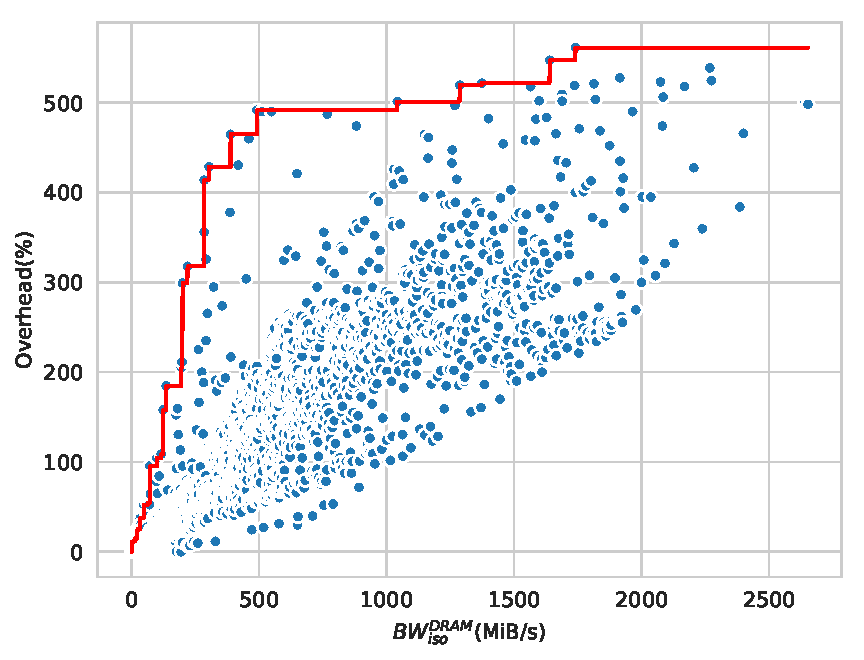
\includegraphics[width=0.65\linewidth]{conservative-inference-bw_dram.pdf}
% 	\caption{\label{fig:conservative-inference}Inférence conservative du surcoût temporel à partir de la bande passante en isolation}
% \end{figure}

% L'inférence illustré dans la figure~\ref{fig:conservative-inference} est certes conservative, mais aussi très imprécise.
% La précision peut être amélioré en considérant d'autres mètriques, mais un problème se pose alors pour construire la fonction de prédiction.
% La fonction que nous avons construite l'est en supposant la monotonie de la fonction associant une bande passante à l'impact des interférences.
% Cela revient à supposer que le consommation de mémoire est une \emph{abstraction} de la sensibilité aux interférences.
% En d'autre termes, si on consomme plus alors on est plus touché par les interférences.
% Si on observe des points invalidant la monotonie, alors on les redresse de manière à la préserver à nouveau.
% Cela suppose de pouvoir \emph{ordonner} les consommations.
% Le problème qui si pose alors est de pouvoir ordonner ces consommations lorsqu'elles sont caractérisées à l'aide de plusieurs variables, tout en conservant la monotonie de l'association avec le surcoût induit par les interférences.